\documentclass[11pt]{article}


\usepackage[sort]{natbib}
\usepackage{bm,amsmath,bbm,amsfonts,nicefrac,latexsym,amsmath,amsfonts,amsbsy,amscd,amsxtra,amsgen,amsopn,bbm,amsthm,amssymb,graphicx}
\usepackage{fancyhdr}
\usepackage[margin=1.0in]{geometry}




\title{Second Monitoring Committee Meeting\\\vspace{4mm} \normalsize{Understanding the Information Content in Diverse Observations of Forest Carbon Stocks and Fluxes for Data Assimilation and Ecological Modeling\\ NERC case partnership with Forest Research}}
\date{\normalsize{3$^{\text{rd}}$ June 2014, \ Room 1L36}}
\author{\normalsize{E. Pinnington}}


\newtheorem{theorem}{Theorem}[section]
\newtheorem*{defn}{Definition}



	
\begin{document}

\maketitle

\section*{Project Background}

A large amount of data is currently being gathered that is relevant to the carbon balance of forests, with much of this data coming from Eddy covariance flux towers \cite{baldocchi2008turner}. Attempts are also being made to combine this data with models of forest carbon stocks and fluxes, such as the Data Assimilation Linked Ecosystem Carbon model (DALEC) \cite{williams2005improved}, in a data assimilation scheme. Currently, however, there are limitations with such schemes as there is a lack of understanding about the additional information provided by different observations. There is also a lack of understanding about observation error correlations. Current data assimilation (DA) schemes for ecosystem carbon flux only specify the diagonal elements of the observation error covariance matrix, $\textbf{R}$, which correspond to the individual uncertainties in particular observations. As such, these DA schemes do not specify observation error correlations or covariances, corresponding to the off diagonal elements of $\textbf{R}$. In numerical weather prediction (NWP) it has been shown that the inclusion of observation error correlations can increase the information content from a given data set and reduce analysis error \cite{stewart2008correlated, stewart2009observation, stewart2013data}. Better understanding of the information content and error correlations of carbon balance observations will form two of the main aims of the project. We begin by introducing the DALEC model which will initially be used to look at the information content in different observations.

\section*{The DALEC model}

The DALEC model is a simple process-based model describing the carbon balance of an evergreen forest ecosystem \cite{williams2005improved}. The model is constructed of five carbon pools (foliage ($C_f$), fine roots ($C_r$), woody stems and coarse roots ($C_w$), fresh leaf and fine root litter ($C_l$) and soil organic matter and coarse woody debris ($C_s$)) linked via fluxes. The gross primary production function ($GPP$) uses meteorological driving data and the site's leaf area index (a function of $C_f$) to calculate the total amount of carbon to be allocated at a daily time step.   
\begin{figure}[h!]
    \centering
    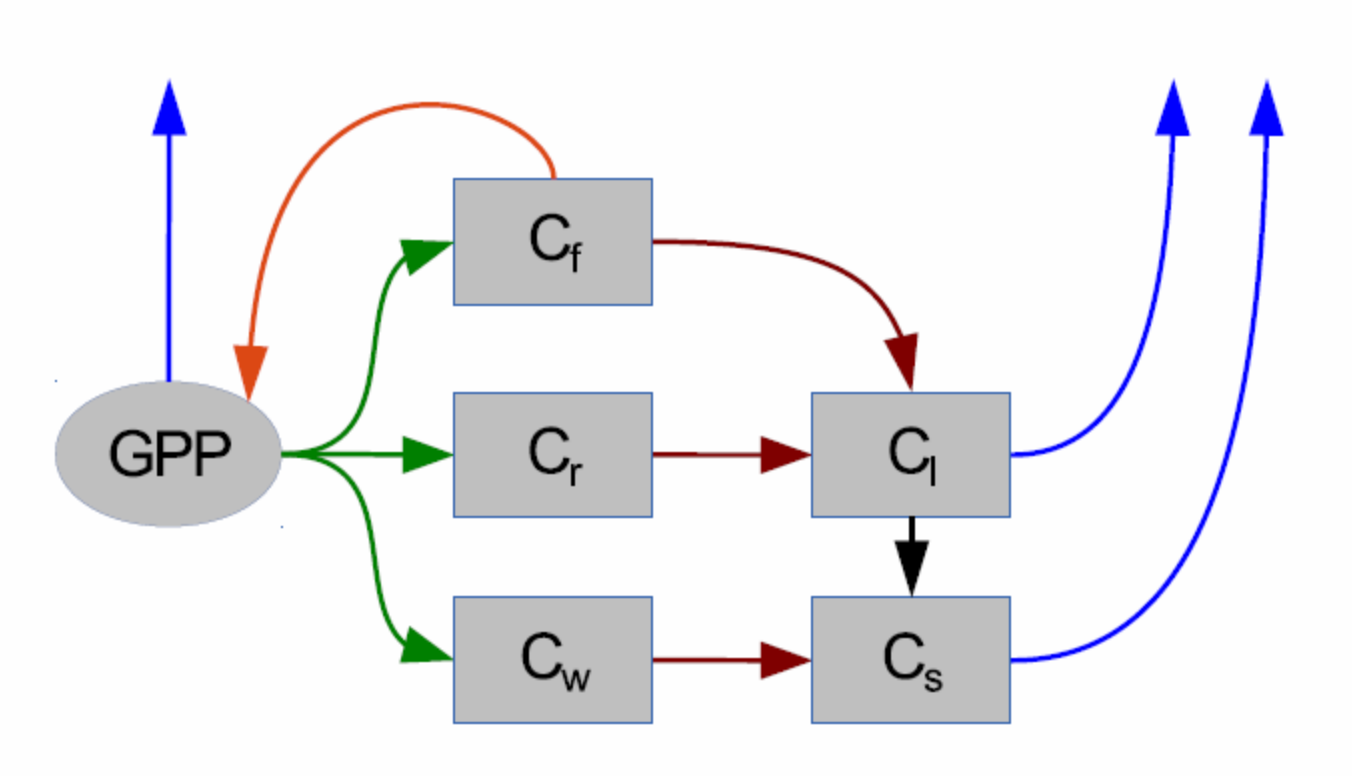
\includegraphics[width=0.5\textwidth]{DALECpic.png}
    \caption{DALEC carbon balance model \cite{delahaies2013regularization}}
    \label{fig:DALEC_mod}
\end{figure}
The model equations for the carbon pools at day $t+1$ are as follows:
%\begin{equation}
\begin{align}
C_f(t+1)&=(1-p_5)C_f(t)+p_3(1-p_2)GPP(C_f(t),\phi),
\\C_r(t+1)&=(1-p_7)C_r(t)+p_4(1-p_3)(1-p_2)GPP(C_f(t),\phi), 
\\C_w(t+1)&=(1-p_6)C_w(t)+(1-p_4)(1-p_3)(1-p_2)GPP(C_f(t),\phi), 
\\C_l(t+1)&=(1-(p_1+p_8)T(t))C_l(t)+p_5C_f(t)+p_7C_r(t), 
\\C_s(t+1)&=(1-p_9T(t))C_s+p_6C_w(t)+p_1T(t)C_l(t),
\end{align}
%\end{equation}
where $T(t)=\frac{1}{2}exp(p_{10}T_m(t))$, $T_m$ is daily mean temperature, $p_1,\ldots,p_{10}$ are rate parameters and $\phi$ represents the meteorological driving data used in the $GPP$ function. The full details of this version of DALEC can be found in \cite{williams2005improved}. We now introduce Shannon Information Content as one method to assess the information content in different carbon balance observations.

\section*{Shannon Information Content and Observation Sensitivity}

In DA Shannon Information Content ($SIC$) is a measure of the reduction in entropy given a set of observations. Entropy physically corresponds to the volume in state space taken up by the probability density function (pdf) describing the knowledge of the state \cite{rodgers2000inverse}. Assuming all pdfs are Gaussian we have,
\[
SIC=\frac{1}{2}ln\frac{\begin{vmatrix} \bf{B} \end{vmatrix}}{\begin{vmatrix} \bf{A} \end{vmatrix}},
\]
where $\bf{B}$ is the background error covariance matrix and $\bf{A}$ is the analysis error covariance matrix. For a larger reduction in uncertainty in our analysis we have a larger value of $SIC$. I began by using $SIC$ to understand the information content for different sets of observations at one time when being assimilated with the DALEC model. We specify the state vector for the assimilation as,
\[ \underline{x}_b = (C_f, C_r, C_w, C_l, C_s)^T, \] 
where the elements of the state vector have variances, $\sigma_{cf,b}^{2},\ldots,\sigma_{cs,b}^{2}$, respectively. We then have the following background error covariance matrix,
\[
\bf{B} = \begin{pmatrix} 
\sigma_{cf,b}^{2} & 0 & 0 & 0 & 0 \\
0 & \sigma_{cr,b}^{2} & 0 & 0 & 0 \\
0 & 0 & \sigma_{cw,b}^{2} & 0 & 0 \\
0 & 0 & 0 & \sigma_{cl,b}^{2} & 0 \\
0 & 0 & 0 & 0 & \sigma_{cs,b}^{2} \\
\end{pmatrix},
\]  
here we assume a diagonal background error covariance matrix. In order to calculate the $SIC$ we need $\begin{vmatrix} \textbf{A}^{-1} \end{vmatrix}$ we have,
\[
\textbf{A}^{-1}=\textbf{J}'' = \textbf{B}^{-1}+\textbf{H}^{T}\textbf{R}^{-1}\bf{H}, 
\]
where $\textbf{J}''$ is the Hessian of $\bf{J}$, the cost function to be minimized in Three-Dimensional Variational Data Assimilation (3D-Var), and $\bf{H}$ is the linearized observation operator. One of the main observations made of the carbon balance of a forest at flux tower sites is the net ecosystem exchange ($NEE$) of CO$_{2}$, which can be estimated by DALEC as the difference between $GPP$ and the respiration of $C_l$ and $C_s$, giving,
\[ 
NEE(t)=-(1-p_2)GPP(C_f(t),\phi)+p_8C_lT(t)+p_9C_sT(t). 
\]
For a single observation of $NEE$ at one time, $t_0$, an analytical expression for the $SIC$ can be derived using,
\[
\textbf{H}_{0} = \begin{pmatrix}
-(1-p_{2})\zeta_0 & 0 & 0 & p_{8}T_{0} & p_{9}T_{0}
\end{pmatrix},
\]  
where $\zeta_0 = GPP'(C_f(t_0), \phi)$, $T_{0}=T(t_0)$ and $\textbf{H}_{0}=\frac{\delta NEE(t_0)}{\delta\underline{x}}$ is the linearized observation operator at time $t_0$. As we have a single observation at one time our observation error covariance matrix, $\bf{R}$, is just the variance of our observation of $NEE$, $\sigma_{nee,0}^{2}$, at time $t_0$. Therefore,
\[
\textbf{R}=\sigma_{nee,0}^{2}
\]  
and
\[
\begin{array} {lcl}
\textbf{J}'' &=& \textbf{B}^{-1}+\textbf{H}^{T}\textbf{R}^{-1}\bf{H} \\
&=& \begin{pmatrix} 
\sigma_{cf,b}^{-2}+\sigma_{nee,0}^{-2}(1-p_{2})^{2}\zeta_0^{2} & 0 & 0 & \sigma_{nee,0}^{-2}(1-p_{2})\zeta_0 p_{8}T_0 & \sigma_{nee,0}^{-2}(1-p_{2})\zeta_0 p_{9}T_0 \\
0 & \sigma_{cr,b}^{-2} & 0 & 0 & 0 \\
0 & 0 & \sigma_{cw,b}^{-2} & 0 & 0 \\
\sigma_{nee,0}^{-2}(1-p_{2})\zeta_0 p_{8}T_0 & 0 & 0 & \sigma_{cl,b}^{-2}+\sigma_{nee,0}^{-2}p_{8}^2 T_0^2 & \sigma_{nee,0}^{-2}p_{8}p_{9} T_0^2 \\
\sigma_{nee,0}^{-2}(1-p_{2})\zeta_0 p_{9}T_0 & 0 & 0 & \sigma_{nee,0}^{-2}p_{8}p_{9} T_0^2 & \sigma_{cs,b}^{-2}+\sigma_{nee,0}^{-2}p_{9}^2 T_0^2 \\
\end{pmatrix}.
\end{array}
\] 
We then have,
\[
SIC=\frac{1}{2}ln\frac{\begin{vmatrix} \textbf{B} \end{vmatrix}}{\begin{vmatrix} \textbf{A} \end{vmatrix}} = \frac{1}{2}ln\begin{vmatrix} \textbf{B} \end{vmatrix}\begin{vmatrix} \textbf{J}'' \end{vmatrix}.
\]
Hence,
\[
SIC = \frac{1}{2}ln\frac{(p_{2}-1)^{2}\zeta_0^{2}\sigma_{cf,b}^{2}+\sigma_{nee,0}^{2}+T_{0}^2(p_{9}^2\sigma_{cs,b}^2+p_8^2\sigma_{cl,b}^2)}{\sigma_{nee,0}^{2}}.
\]
If we assume that the variances and parameters here are fixed we can see that the size of the $SIC$ is dependent on the temperature term, $T_0$, and the square of the first derivative of $GPP$, $\zeta_0^{2}$. Generally, the value of $GPP$ (and its first derivative) is highest in summer with higher total daily irradiance and higher temperatures. We therefore have that there will be more information content in observations that are taken when temperatures are higher. **Physically this makes sense as more NEE takes place when temperatures are higher (to a point) so measurements are of greater magnitude and give us more information of carbon fluxes**. I have also derived analytical forms for the $SIC$ using different sets of observations at a single time, which all have a similar form.

Following this work, based at a single time, I started looking at the $SIC$ when successive observations are added over a period of time. The model was now built into a Four-Dimensional Variational Data Assimilation (4D-Var) framework where our observation operator, $\textbf{H}$, and observation error covariance matrix, $\textbf{R}$, are now,
\[ 
\textbf{H}=
\begin{pmatrix}
\textbf{H}_0 \\
\textbf{H}_1\textbf{M}_0\\
\vdots \\
\textbf{H}_n\textbf{M}_{n,0}
\end{pmatrix}
\hspace{5mm} \text{and} \hspace{5mm}
\textbf{R}=
\begin{pmatrix}
\textbf{R}_0 & 0 & 0 & 0 \\
0 & \textbf{R}_1 & 0 & 0 \\
0 & 0 & \ddots & 0 \\
0 & 0 & 0 & \textbf{R}_n
\end{pmatrix},
\]
where $\textbf{H}_i$ is our linearized observation operator at time $t_i$, $\textbf{M}_{i,0}=\textbf{M}_{i-1}\textbf{M}_{i-2}\cdots\textbf{M}_0$ is our linearized model evolving the state vector, $\underline{x}_b$, at time $t_0$ to time $t_i$ and $\textbf{R}_i$ is the observation error covariance matrix corresponding to $\textbf{H}_i$ at time $t_i$ \cite{lewis2006dynamic}. I first calculated the adjoint model for DALEC analytically as $\textbf{M}_i=\frac{\delta \underline{m}_i}{\delta \underline{x}_i}$. I then wrote a code in Python that calculates $\textbf{H}$ and $\textbf{R}$ to find a value of $SIC$ when successive observations of $NEE$ are made each day over a chosen period (To calculate the $SIC$ we do not need the actual observation value). The meteorological driving data used in the model is taken from a Ponderosa pine forest in central Oregon for which the DALEC model in \cite{williams2005improved} is parameterized. Below we have a plot when different starting points and periods are chosen, day 0 represents the start of the year so that day 200 is the 19th of July.

\begin{figure}[ht]
\centering
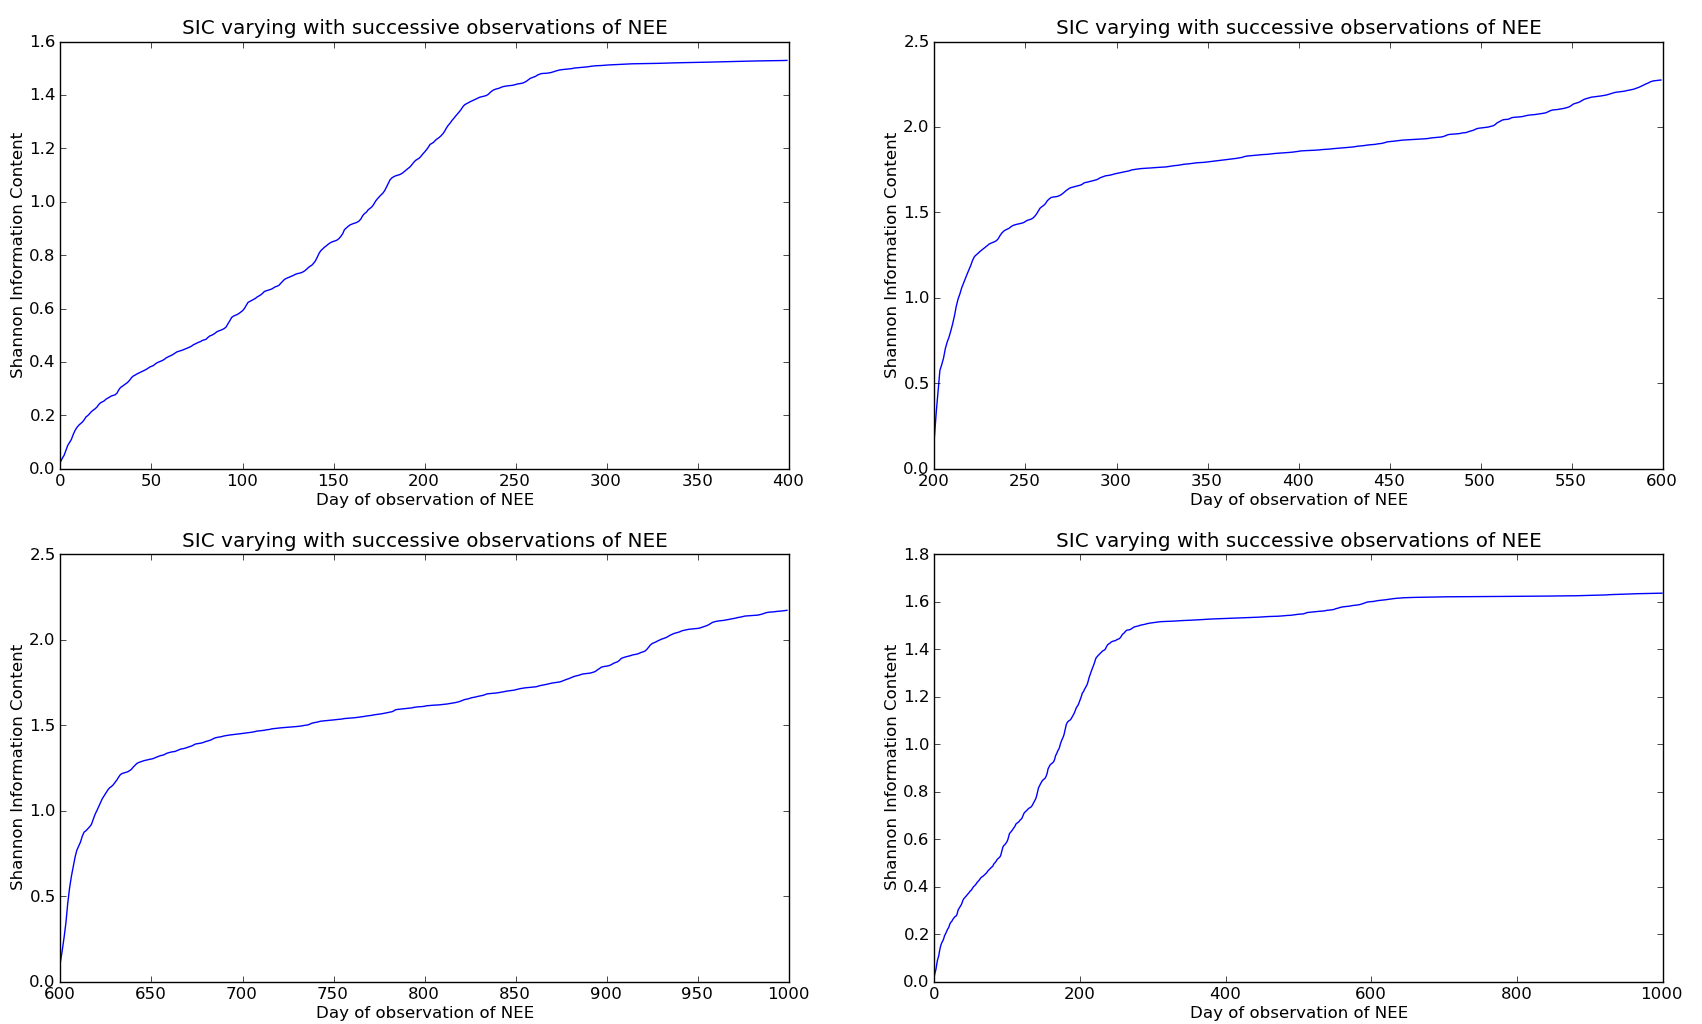
\includegraphics[width=1\textwidth]{SICsubplot.png}
\caption{$SIC$ varying as successive observations of $NEE$ are added using driving data from Oregon pine forest.}
\label{fig:SIC_subplot}
\end{figure}

When starting at day 0 we can see a leveling off in the $SIC$ after 200 days of observations when the forest in Oregon will be experiencing  some of the highest temperatures of the year. When starting our observations from day 200 we see that the $SIC$ levels off much quicker and achieves a higher value than the first period. This agrees with the analytic form of $SIC$ found previously for a single observation that is a function of temperature. The reason for the leveling off of the $SIC$ when yearly peak temperatures are reached  needs to be investigated further. **As temperatures decrease very little information is added to the system, see graph of single observations of NEE as opposed to successive observations of NEE (make this graph if this hasnt been done!).**
%We now run the same code using the mean driving data so that the temperature is the same on every day.
%\begin{figure}[ht]
%\centering
%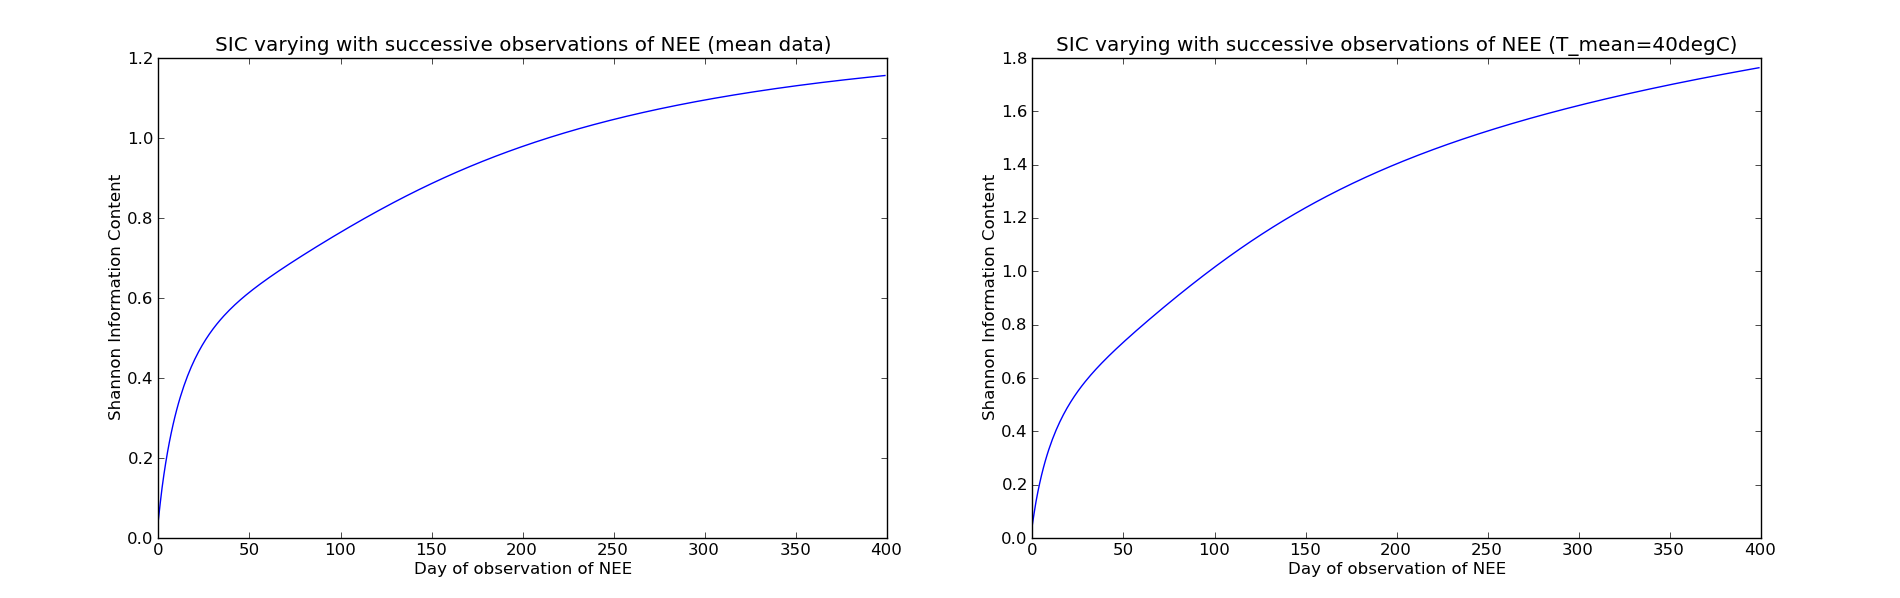
\includegraphics[width=1\textwidth]{SICmeandatasubplot0_400.png}
%\caption{$SIC$ varying as successive observations of $NEE$ are added using mean driving data and data with constant temperature of $40^oC$ from Oregon pine forest.}
%\label{fig:SICmean_subplot}
%\end{figure}
%\newpage
%Here we still have the $SIC$ leveling off at around day 200 however if instead of using the mean data we specify a temperature of $40^oC$ as the temperature used for every %observation of $NEE$ our $SIC$ levels off at around day 150. To investigate the leveling off in $SIC$ further we look at the error in our linearized DALEC model. 

\section*{Error in the Linear Model}

**Redo this with correct GPP'**
It is important to understand how well our linearized model performs. In 4D-Var we use our linearized model in the approximation,
\[ m(\underline{x}+\delta \underline{x}) \approx m(\underline{x}) +\textbf{M}\delta \underline{x}, \]
where $m(\underline{x})$ is our non-linear model applied to the state $\underline{x}$. To see if this approximation is reasonable we can plot,
\[ \delta\underline{x}_N = m(\underline{x} + \delta\underline{x})-m(\underline{x})
 \hspace{5mm} \text{and} \hspace{5mm}
 \delta\underline{x}_L = \textbf{M}\delta \underline{x} \]
using the initial conditions for the carbon pools given in \cite{williams2005improved} as our state, $\underline{x}$, and a value of 10\% of each pool for our perturbation $\delta\underline{x}$. If we then run our linear and nonlinear models forward over 1000 days using these initial conditions and plot $\delta\underline{x}_N$ and $\delta\underline{x}_L$ we will be able to see how well our linear DALEC model performs.
\begin{figure}[ht]
\centering
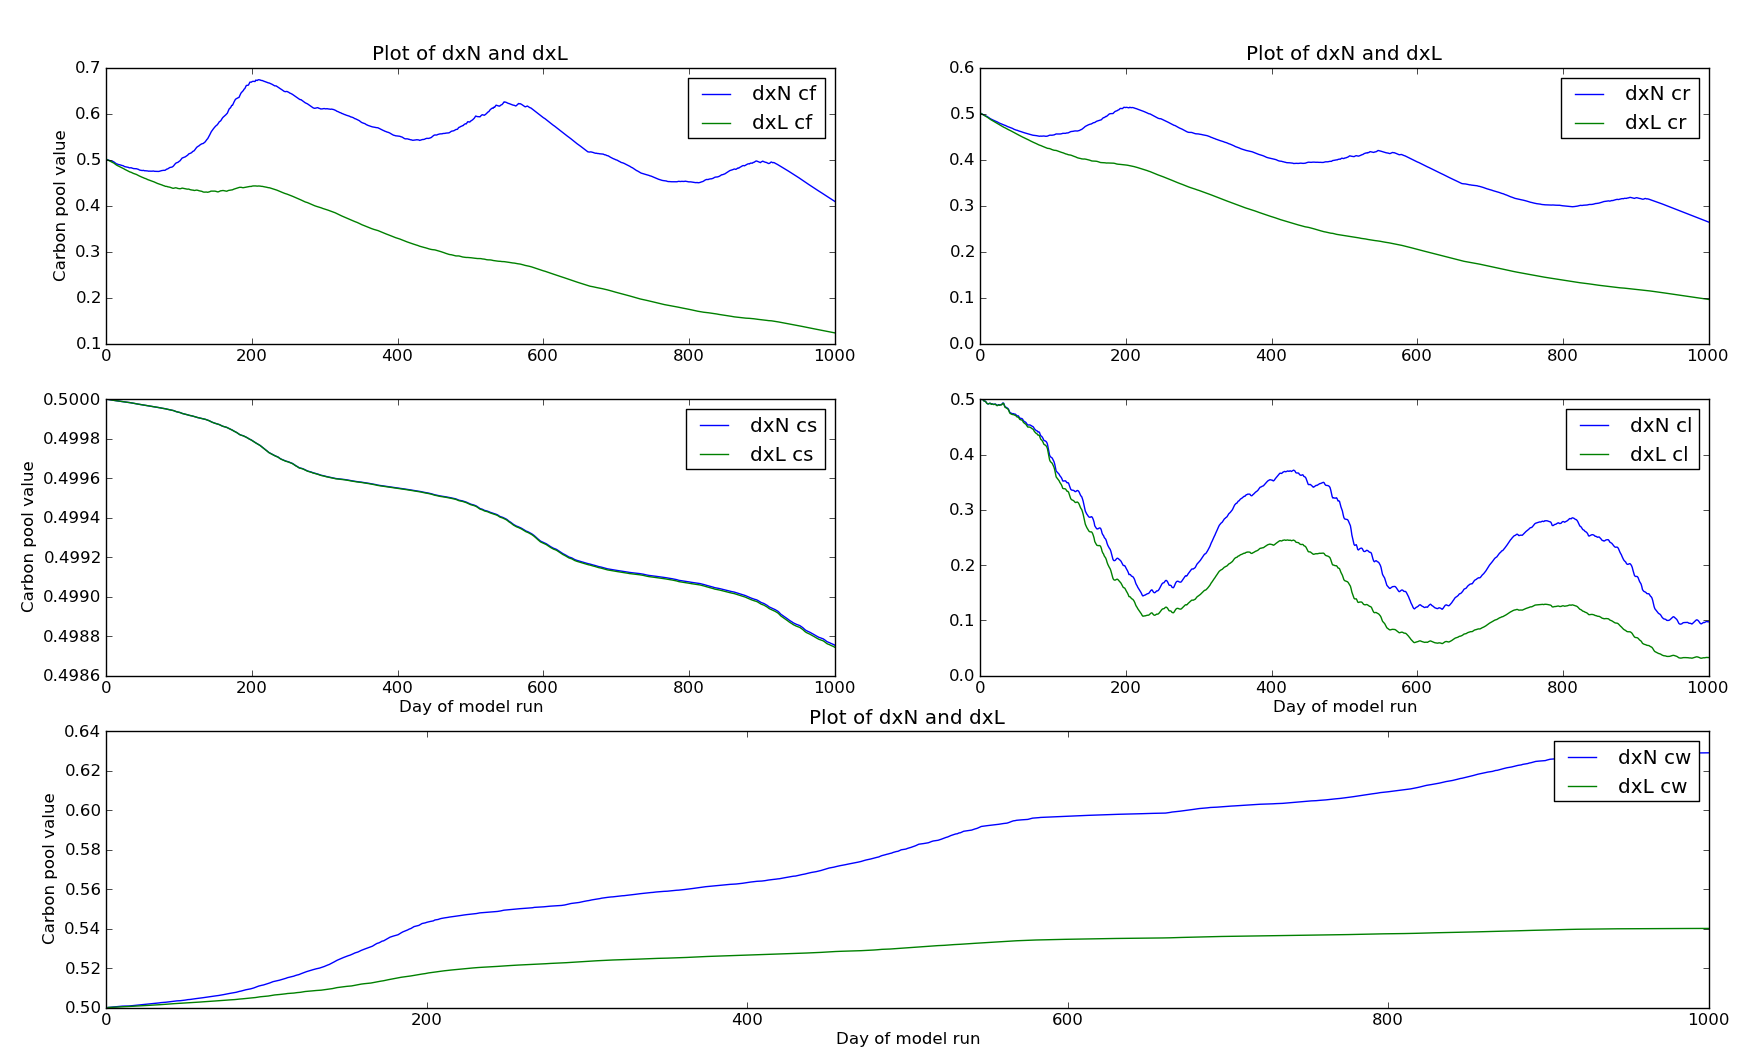
\includegraphics[width=1\textwidth]{dxNdxLCpoolsubplot2.png}
\caption{Plot of $\delta\underline{x}_N$ and $\delta\underline{x}_L$ for each of the carbon pools in the state $\underline{x}$}
\label{fig:dx_subplot}
\end{figure}
%\newpage
Here then we see that although the linear model is a very good approximation for $C_s$ the other pools diverge considerably by day 1000, with approximately a $70\%$ error in $C_f$ and a $15\%$ error in $C_w$. This shows that past day 100 our linear approximation for the DALEC model does not perform well.

\section*{Future Plans}

My plans for the future are as follows:

\begin{itemize}
\item I will continue to investigate the reason behind the leveling off in $SIC$ for successive observations of $NEE$ and its relation to temperature. When this is understood I will start investigating the $SIC$ for different sets of observations over a period of time to understand if there is an optimal set of observations or an optimal time to make a set of observations for the DALEC model. I will also begin looking at the `degrees of freedom for signal' \cite{rodgers2000inverse} as another measure of information content.

\item I have begun building DALEC into an operational DA scheme using the meteorological driving data from the forest in Oregon. The data also contains observations of forest carbon balance to be assimilated with the DALEC model. Once I have a fully working DA scheme for DALEC I shall start using the Desroziers diagnostics in an attempt to find a correlated $\textbf{R}$ \cite{desroziers2005diagnosis}. Once we have a better specified $\textbf{R}$ I will repeat the information content experiments to see what effect using this new $\textbf{R}$ has. I will also undertake more reading in the area of correlated observation errors and hopefully find a way to build some temporally correlated errors into $\textbf{R}$ as opposed to just correlations between observations taken at the same time.  

\item In the next academic year I will begin spending time at the Forest Research site Alice Holt, this will allow me to see how different forest carbon balance observations are actually taken. I will also develop an understanding of the constraints on when and how many observations can be made so that I do not conduct unrealistic information content experiments.  

\item I will start reading up on other forest carbon balance models and possibly begin working with the the Simplified Photosynthesis and Evapo-Transpiration model (SiPNET) \cite{braswell2005estimating}. I will then try to apply the techniques I will have built up with DALEC to these more complicated models.
\end{itemize}

\section*{Professional and Academic Development}

\subsection*{Masters Courses}
I have now completed the seven masters courses in which I was enrolled at the beginning of the first term. In my first term module I received the following marks:
\begin{itemize}
\item MAMB10 (Data Assimilation) - 85\%
\item MAMNSO (Numerical Solutions to Ordinary Differential Equations) - 79\%
\item MTMG02 (Atmospheric Physics) - 66\%
\end{itemize}
Computing techniques and projects was taken as just a formative module with no assessment. I have taken all the exams for my three second term modules (MTMG49 - Boundary Layer, MTMD01 - Environmental Data Visualization and Exploration, MTMD02 - Operational Data Assimilation) and am awaiting the results. 

\subsection*{Transferable Skills}

During my PhD I have taken part in the following courses:
\begin{itemize}
\item 28/01/2014 - Basic Statistics Refresher - RRDP

\item 31/03/2014-01/04/2014 - Land Data Assimilation workshop at UCL - ESA

\item 23/04/2014-25/03/2014 - Correlated Observation Errors in Data Assimilation - ESA

\item 13/05/2014 - Social Media - Bloggs, Twitter and Your Online Presence - RRDP
\end{itemize}
In the coming months I will be attending:
\begin{itemize}
\item 29/05/2014 - How to Write a Paper - RRDP
\item 21/07/2014-01/08/2014 - Fluxcourse - University of Colorado
\item 25/06/2014-26/06/2014 - Software Carpentry - Git and Python
\item 10/07/2014-11/07/2014 - Forest Research - Helped with field work LiDAR 
\end{itemize}
The Fluxcourse is held in Boulder Colorado and I hope it will help me see the problems in my project from a different view point as I have come from a mathematics degree and the course is taught by some of the leading scientists in the field of forest carbon balance.  


\bibliography{../../PhD}{}
\bibliographystyle{plain}
\end{document}
